\subsection{Shielding}

Effective shielding is of great interest to reduce EMI of electronic systems. A figure of merit for shielding capabilities of a material is the electromagnetic shielding effectiveness (SE), given in \autoref{eqn:se_elec_fields} \cite{10518640}. $E_\mathrm{i}$ is the incident electric field, while $E_\mathrm{t}$ is the transmitted electric field, also depicted in \autoref{fig:shielding_material_diagram}. It depends on the thickness and shape of the material, and its electric and magnetic properties. Addtionally, the TEM cell contributes to the SE values.

\begin{equation}
    SE_{\mathrm{dB}}=20\log{(\frac{E_\mathrm{i}}{E_\mathrm{t}})}
    \label{eqn:se_elec_fields}
\end{equation}

\begin{figure}[h]
    \centering
    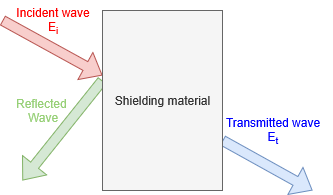
\includegraphics[width=0.35\linewidth]{Documentation//images/shielding_material_diagram.png}
    \caption{Incident, reflected and transmitted electric fields due to interaction with shielding material}
    \label{fig:shielding_material_diagram}
\end{figure}

Note: Higher order modes may not be able to propagate in the TEM cell, as the refraction of the shielding material follows to excitation of these modes.

% Quick mathematical formulation of how to calculate reflected waves?
